\chapter{Basic Neuroscience}\label{ch_neuro}
\chapterauthor{Jeff Yoshimi, Chelsea Gordon, David C. Noelle}{.4,.4,.2}

% Talk about inhibitory/excitatory ratios.   Esp since the sparse connectivity thing.  Also http://www.scholarpedia.org/article/Balance_of_excitation_and_inhibition which has this line, which begins to resolve the mystery a bit; “The possibility of excitation and inhibition having a comparable strength might seem implausible at first, since interneurons comprise only 15% - 25% of the population of cortical neurons. However, the synaptic strength and firing rates of inhibitory interneurons are substantially higher than in excitatory neurons, thus inhibitory interneurons have an impact disproportionate to their relatively small number.”

% https://cs.stanford.edu/people/karpathy/convnetjs/ interactive. but find something better

In this chapter, we review the basic physiology of neurons and synapses, which are the basis of equations describing how node activations and weight strengths change. We also provide an overview of the major circuits of the brain, reviewing their basic features, and giving a sense of how these circuits are understood from a neural networks standpoint.\footnote{Some useful general references include Kandel (2000) \cite{kandel2000principles} and Gazzaniga (2002) \cite{gazzaniga2002cognitive}. An outstanding online source is \url{https://science.eyewire.org/home}. A detailed book length treatment of the topics outlined in this chapter is \cite{cecn_4e}, which has also been developed into a free online text supported by open source software: \url{https://compcogneuro.org/}.}  

\section{Neurons and synapses}\label{neuronsSynapses}

\subsection{Neurons}

Neurons are brain cells, which have all the machinery any cell has: mitochondria, Golgi apparatus, a nucleus whose DNA is actively expressing genes, and a membrane studded with an array of proteins. Neurons communicate using a finely orchestrated pattern of electrical, chemical, and molecular processes. Neural network models typically abstract from most of these details. Classical neural network models only simulate certain high level features of the way information is transmitted from one neuron to another. Models in computational neuroscience (described in chapter \extref{ch_intro}) capture more of the biological details, but still abstract away from many features of real neurons. In the next two sections we give a rudimentary overview of the structure of neurons and synapses, focusing on features that are commonly referenced in neural network models.

\begin{figure}[h]
\centering
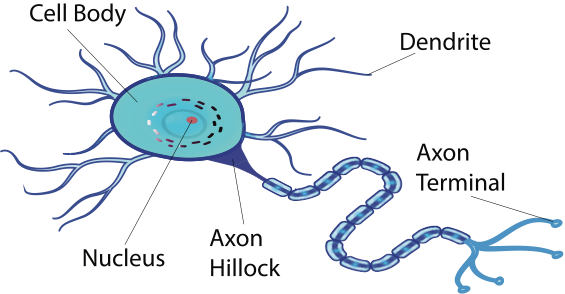
\includegraphics[width=.5\textwidth]{./images/neuron.png}
\caption[Pamela Payne.]{Main structures of a neuron.}
\label{f:neuron}
\end{figure}

% Possibly add discussion of myelin sheath, fast cortico-cortical communication, and white vs. gray matter
Most neurons have dendrites, axons, and a cell body (see Fig. \ref{f:neuron}).\footnote{There are many types of neurons in the brain, but in this section we focus on the \emph{multipolar} neuron. This type of neuron has one axon and multiple dendrites, which allows it to receive information from many other neurons. Other types of neuron include unipolar and bipolar neurons.}  These are not really distinct structures, but are parts of the cell. The neuron as a whole is a kind of container, whose overall charge is changing constantly over time like a fluctuating battery or capacitor. 

\glossary{Dendrites} are extensions that grow out of the cell body like a tree (``dendrite'' comes from a Latin word that means ``tree''). This is where information-carrying chemicals are received from other neurons. Dendrites have small branches, which can receive signals from many other neurons. Some metaphors might help you remember this: You can think of a dendrite as the mail-box of a neuron, receiving messages from many nearby cells. You can also think of it as a catcher's mitt, since it receives or ``catches'' inputs from other neurons.

% Maybe say more about what's happening in the cell body. Expressing genes to produce and package and transport neurotransmitter, for example. Just a flavor of how active it is. 
The cell body or \glossary{soma} is home to many organelles that work to produce and package proteins for the cell. These proteins have a variety of important functions, including the production of neurotransmitters that signal between cells. The soma sums together all the information gathered from the dendrites. If the voltage changes enough at a part of the soma called the \emph{axon hillock}, the neuron will fire an \glossary{action potential} or spike along its axon. We expand on these ideas in the discussion of synapses next. 
% [Merge or make footnote] These chemicals are called \glossary{neurotransmitters}. These messages (neurotransmitters) attach themselves to \glossary{receptors} on the dendritic branches. Different types of neurotransmitters have different binding sites on the dendrite. Once attached, these chemical messages trigger the electrical transmission of ions throughout the rest of the cell. The particular message carried by a neurotransmitter is important for determining what happens inside of the cell once it binds, and we will discuss a bit later what these different types of messages are. Importantly, this transmission changes the voltage of the cell as a whole, and as we will see, this voltage change is an important  component of within-neuron communication.

The \glossary{axon} is another extension growing out of the cell body. Axons can be different lengths, but they often have a long main extension terminating in a branched structure. When the neuron fires an action potential, electrical activity propagates down these extensions and triggers the stimulation of the dendrites of other neurons. Continuing our metaphors: the terminals at the end of the axons can be thought of as a neuron's post office, where the ionic messages transmitted down the axons are packaged into neurotransmitter chemicals and sent out on their route to the receiving neuron's dendrite. Or, continuing the baseball metaphor, the axon is like the arm of a pitcher, throwing signals to other dendrites, which catch them.\footnote{Fast communication between long-distance neurons is made more efficient by a fatty white substance, called \emph{myelin sheath}, that wraps around the axons of neurons and insulates them, allowing better conduction of electrical signals}

% Mention Simbrain and all the neuron models it contains. Point ahead to next chapter.

\subsection{Synapses and neural dynamics}\label{simpleNeuralDynamics}

Communication between neurons happens at a \glossary{synapse}, which is a junction where the axon of the \emph{pre-synaptic} neuron almost touches the dendrite of the \emph{post-synaptic neuron}, often at a protrusion called a \emph{dendritic spine}. See Fig. \ref{f:synapse}.\footnote{There are two types of synapses, electrical synapses and chemical synapses. Electrical synapses, instead of having a cleft between the post- and pre-synaptic neurons, have a much smaller space called a \emph{gap junction}, which connects the pre-synaptic neuron directly with the post-synaptic neuron, allowing for electrical communication. These synapses allow neurons to fire in synchrony and are important for quick communication between neurons. However, most communication happens via chemical synapses, which transmit much stronger signals and have more permanent effects. The main text focuses on chemical synapses.}  When an action potential reaches the axon terminal of the pre-synaptic neuron, chemicals called \glossary{neurotransmitters} are released into the synaptic cleft. These neurotransmitters are housed in water-balloon-like containers called \emph{vesicles}. The vesicles fuse into the pre-synaptic cell membrane when an action potential occurs, releasing their neurotransmitters into the synaptic cleft. The neurotransmitters then bind to \glossary{receptors} on the post-synaptic neuron. This is like a key being fit into a keyhole--the neurotransmitters are the keys and the receptors are the keyholes which, when opened, let ions (charged particles) flow in to the post-synaptic dendrite. These ions are negatively or positively charged, and the balance between the total charge of these ions on either side of the cell membrane is what is called the \glossary{membrane potential}.\footnote{This charge is maintained by ion channels that selectively let some ions travel into and out of the cell. Some of these ion channels are called \emph{passive ion channels}, which stay open and allow the constant light flow of Na$^+$ and K$^+$ ions through the cell membrane. There are also \emph{gated ion channels}, which are those that open during an action potential and cause a much larger exchange of ions. When these open, the ions released cause changes in the membrane potential of the post-synaptic neuron.}

\begin{figure}[h]
\centering
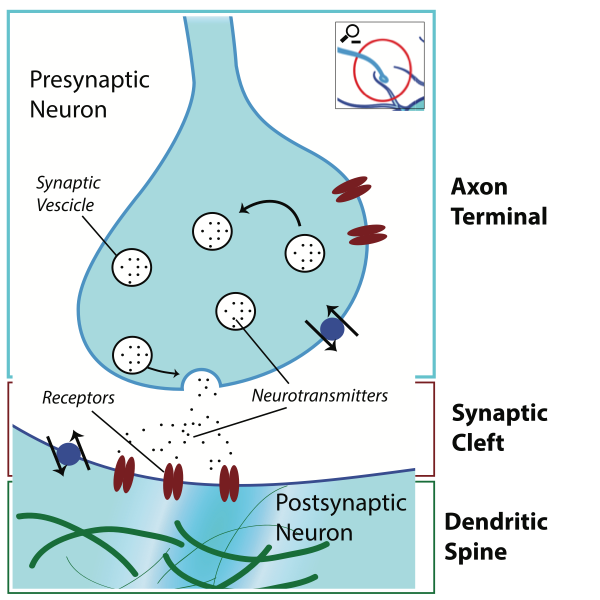
\includegraphics[width=.45\textwidth]{./images/synaptic_cleft.png}
\caption[Pamela Payne.]{Some structures associated with a synapse.}
\label{f:synapse}
\end{figure}

There are different kinds of synapses. The pre-synaptic neurons of  \glossary{excitatory synapses} release neurotransmitters, which result in the  post-synaptic voltage being raised, which makes it more likely that an action potential will occur post-synaptically. \emph{Glutamate} is one of the most common excitatory neurotransmitters. \glossary{Inhibitory synapses} release neurotransmitters, which result in the voltage being lowered post-synaptically, and make it less likely that an action potential will occur post-synaptically. \emph{GABA} is the most common  inhibitory neurotransmitter.

\begin{figure}[h]
\centering
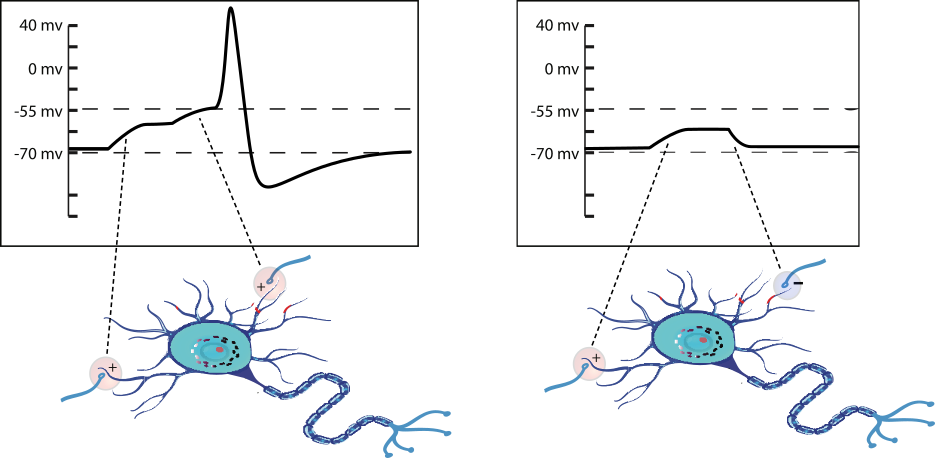
\includegraphics[scale=1.5]{./images/membranePotential3.png}
\caption[Adapted from original work by Pamela Payne.]{(Left) Two successive excitatory inputs increase the neuron's membrane potential beyond the threshold potential, after which it fires an action potential. (Right) First an excitatory input increases the neuron's membrane potential, then an inhibitory input reduces it. }
\label{membranePotential}
\end{figure}
% Make blue darker

A neuron can receive both excitatory and inhibitory inputs.\footnote{What we are calling excitatory and inhibitory inputs are actually synaptic events that allow ions to rush in or out of the cell, and thus produce excitatory or inhibitory currents. From this standpoint the neuron is like a battery or capacitor and its membrane dynamics can be understood in terms of circuits (the ``Rall model'' or ``cable theory'' of the neuron), which can be precisely described in computational neuroscience models. The membrane potential has an average resting state, usually around -70 mV, which is the difference between the electrical charge inside and outside of the membrane when a neuron is at rest. Excitatory and inhibitory inputs alter this resting state. One metaphor that helps here is that of a tank of water or a graduated cylinder, where the level of water represents the current voltage potential. There is a hole on the side of the tank that constantly lets some water out, and a tube above it that constantly lets some water in. These produce a ``leak'' current that balances out to a certain standing level in the tank, which is like the resting potential of a cell. That level is roughly where the hole on the side of the tank is. Excitatory inputs briefly open up additional tubes above the tank, letting more water in and raising the water level (the membrane potential), and inhibitory inputs briefly open up additional tubes below the tank, letting more water out and reducing the water level. These transient events lead to fluctuations in the water level which correspond to sub-threshold dynamics of the membrane potential.} As different axons attaching to a neuron release excitatory neurotransmitters (like glutamate) and inhibitory neurotransmitters (like GABA), the binding of neurotransmitters to receptors on the post-synaptic neuron causes ion channels to open and close, letting different ions in and out. As a result, the neuron's voltage goes up and down. When the voltage at the axon hillock passes a specific membrane potential called the \glossary{threshold potential}, an action potential is fired. The process is illustrated in Fig. \ref{membranePotential}. In the left panel, two excitatory synapses are activated successively, and the membrane potential is increased each time until it passes the threshold potential and an action potential is fired.\footnote{Notice the signals occur at spatially distinct dendrites and at different points in time, and that they have a cumulative effect on the membrane potential at the soma. This is known as \emph{spatial and temporal summation}.}  In the right panel, first an excitatory synapses is activated, which raises the membrane potential, and then an inhibitory synapse is activated, which reduces the membrane potential, in effect turning off or ``shunting'' the impact of the first excitatory input, so that no action potential occurs. Changes in membrane potential due to excitatory and inhibitory events that occur below threshold are sometimes referred to as sub-threshold dynamics.

As more excitatory signals are received, the membrane potential will exceed the threshold potential more often, and action potentials will begin to occur more frequently. Thus we can represent the overall activity of a cell in terms of its \glossary{firing rate}, which is measured in number of spikes per unit time, usually spikes per second. A highly ``active'' neuron is one that produces many spikes per second (e.g. 200 Hertz, which is 200 times per second), while a more dormant or quiescent neuron might only produce a few spikes per second (e.g. 2 Hertz). In a time series plot of such a neuron's membrane potential, spikes for a highly active neuron are close together; for a less active neuron they are farther apart. You can get a feel for this in the Simbrain simulation  \emph{spikingNeuronTwoInputs.zip}. In the simulation you can increase the firing rate of the neuron on the left by raising the excitatory input. You can then reduce its firing rate by raising the inhibitory input. See figure \ref{twoNeuronsSpiking}.
  
 \begin{figure}[h]
\centering
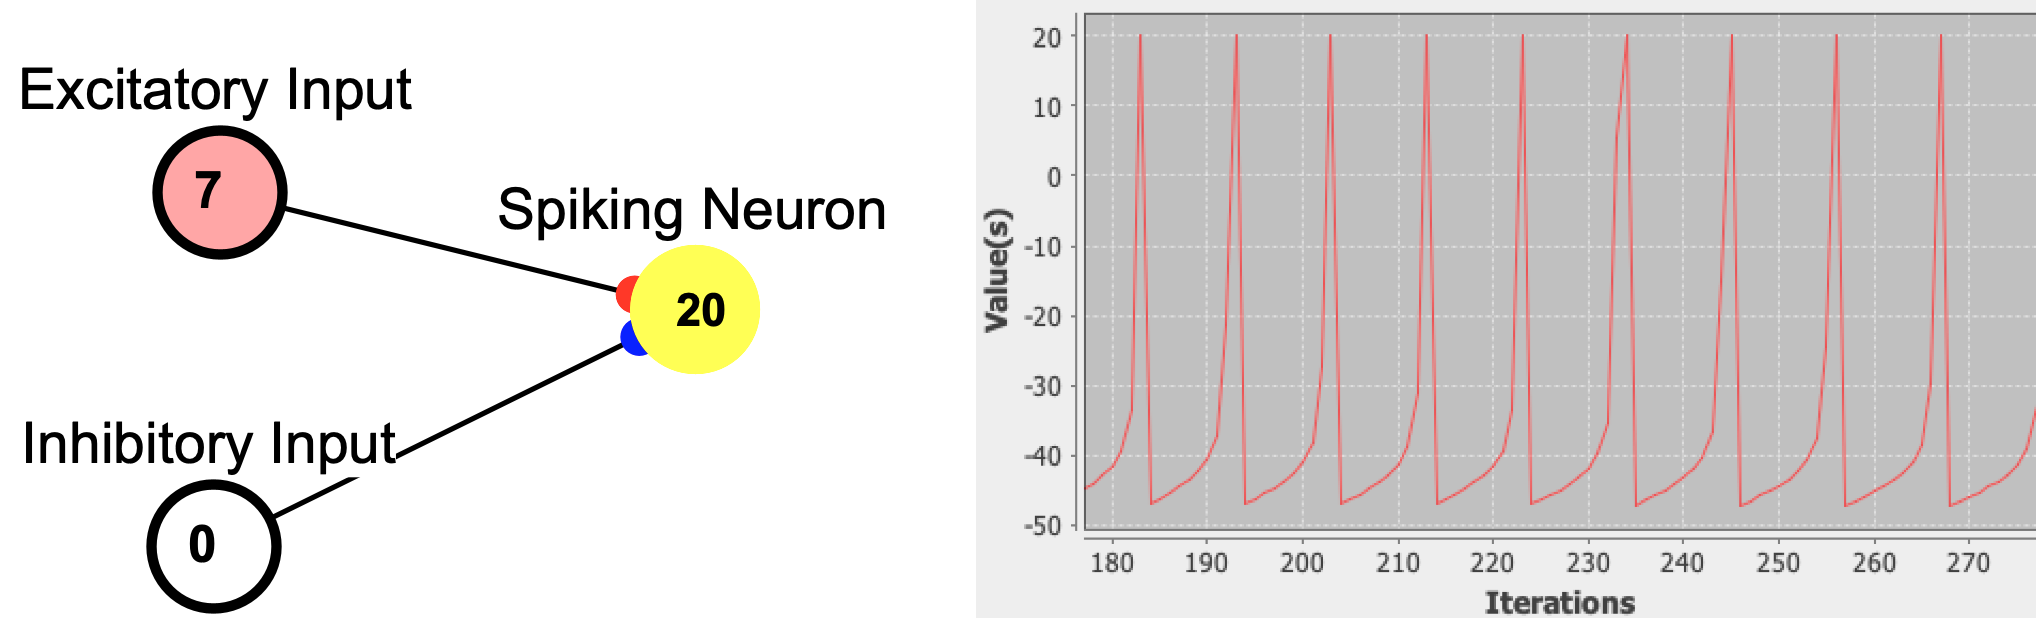
\includegraphics[scale=.4]{./images/TwoNeuronsSpiking.png}
\caption[Jeff Yoshimi.]{(Left) A Simbrain simulations that illustrates how different combinations of excitatory and inhibitory inputs produce different firing rates in an output neurons. As the excitatory input is increased, the firing rate increases, and as inhibitory input is increased, the firing rate decreases. The output neuron is in the middle of a spike at the moment shown. }
\label{twoNeuronsSpiking}
\end{figure}
% The rate coding idea that the number _represents_ that rate is not yet clear, but not sure how much an be done here

These observations are the basis of ``rate-coding'' models. In these models, the number in a node represents a neural firing rate. Weights in these models capture the idea the neuron sums together excitatory and inhibitory signals. Rate coding is in the background of many connectionist models, where much of the biology is abstracted away and all that is maintained is the general idea that a weighted sum of inputs determines the output of a node.  More complex computational neuroscience models describe the changing membrane potential directly, or simulate the action potential using discrete spiking events (see chapter \extref{ch_spiking}). These models are discussed in the chapter on computational neuroscience and in the chapter on classical nodes and weights.

Synapses are modifiable. For example,  \glossary{Long Term Potentiation} or LTP occurs when certain synapses transmit information repeatedly in a short time. When this happens the synapse is ``strengthened'': when an action potential reaches the same synapse after LTP has occurred, the post-synaptic response will be greater than it was before.\footnote{The details of LTP are not well understood, but roughly what happens is this: the repeated stimulation of the post-synaptic neuron results in an influx of calcium ions, which has a number of effects. One is the recruitment of additional receptors to the post-synaptic dendrite, so that when neurotransmitters are subsequently released into the synaptic cleft more receptors open and more ions are allowed into the post-synaptic cell.}   Long term potentiation is the basis of the Hebb rule, discussed in chapters \extref{ch_history} and \extref{ch_unsupervised}. The basic idea of the Hebb rule is that ``neurons that fire together, wire together.''\footnote{This can be visualized in several Simbrain simulations, for example \emph{autoassociator1.zip} and \emph{autoassociator2.zip} in the courseMaterials directory.}   

Synapses can be modified in other ways. Sometimes synapses are weakened via a process of \emph{Long term depression} or LTD. Synapses can be modified in other ways as well, and the study of synaptic plasticity is a major area of research. These changes in synaptic efficacy are thought to be the basis of most forms of learning in humans and animals. The idea that changing connection strengths are the basis of learning is what gives ``connectionism'' its name, and is fundamental to neural network theory.

\subsection{Neuromodulators}\label{neuroModulator}

% https://www.ncbi.nlm.nih.gov/pmc/articles/PMC5807333/
% The cerebrospinal fluid (CSF) occupies the brain’s ventricles and subarachnoid space and, together with the interstitial fluid (ISF), forms a continuous fluidic network that bathes all cells of the central nervous system (CNS). As such, the CSF is well positioned to actively distribute neuromodulators to neural circuits in vivo via volume transmission. Recent in vitro experimental work in brain slices and neuronal cultures has shown that human CSF indeed contains neuromodulators that strongly influence neuronal activity. 

We mentioned GABA and glutamate above. These are neurotransmitters that support local communication from one neuron to another. Other neurotransmitters---which are sometimes called ``neuromodulators''---are connected with circuits that project across larger regions of the brain and have longer-lasting impacts.\footnote{On the relationship between neurotransmitters, neuromodulators, and neurohormones  ``A neurotransmitter is a messenger released from a neuron at an anatomically specialised junction, which diffuses across a narrow cleft to affect one or sometimes two postsynaptic neurons, a muscle cell, or another effector cell. A neuromodulator is a messenger released from a neuron in the central nervous system, or in the periphery, that affects groups of neurons, or effector cells that have the appropriate receptors. It may not be released at synaptic sites, it often acts through second messengers and can produce long-lasting effects. The release may be local so that only nearby neurons or effectors are influenced, or may be more widespread, which means that the distinction with a neurohormone can become very blurred. A neurohormone is a messenger that is released by neurons into the haemolymph [or, in mammals, into the blood] and which may therefore exert its effects on distant peripheral targets.'' \cite{burrows1996neurobiology}.}   Some neural network simulations model the effects of these neurotransmitters.

\emph{Norepinephrine}, or noradrenaline, is produced by neurons in the brainstem and broadcast throughout the brain. It regulates arousal: there is a greater amount of norepinephrine when awake and a decreased amount while asleep. 

\emph{Serotonin} is also produced by cells in the brainstem. Serotonin is involved in attention and complex cognitive function. Low serotonin has been linked to depression. A type of medicine referred to as an SSRI (selective serotonin reuptake inhibitor) causes less of the serotonin released by cells to be taken back into the pre-synaptic neuron, so that more serotonin stays in the synapse and gets used. 

\emph{Acetylcholine}, found in motor neurons in the spinal cord, is responsible for movement and also mediates certain forms of plasticity. Too little acetylcholine can inhibit movement, while too much acetylcholine can cause twitching. Black widows inject a chemical in their bite that promotes the release of acetylcholine, which leads to severe muscle twitching.

\emph{Dopamine} is a neurotransmitter produced in the basal ganglia (in the ``nigrostriatal pathway''), which plays an important role in controlling movement. Shortage of dopamine in the system can lead to \emph{Parkinson's disease}, characterized by an inability to initiate movements. A drug called \emph{L-Dopa} can be used to stimulate the production of dopamine, which helps to even out dopamine levels and alleviate some of the symptoms exhibited by Parkinson's patients. Dopamine is also important in regulating the reward-based learning that occurs in the basal ganglia, which is discussed further below.  It is important to note that dopamine is \emph{not} a direct signal of reward (that signal is carried by other opioid-based circuits in the brain), but rather a signal of how much more or less reward than expected was obtained; a kind of error signal.  When things are going better than expected, dopamine neurons fire at an increased rate.  When things are going worse, they fire at a reduced rate. When you are not expecting a donut (assuming you like donuts and are hungry), the arrival of a delicious donut will cause dopamine neurons to start firing. But as you eat, even if you are still hungry, dopamine neurons stop firing, because your expectations are no longer changing.  On the other hand, if you were expecting those donuts when the door opened and you are disappointed to see that your friend forgot to bring them (oh the horror), your dopamine neurons will fire \emph{less} than normal. Thus dopamine is an important signal which can be used to train animals, by encouraging them to do things that lead to unexpected rewards, and by discouraging them from doing things which lead to unexpected disappointment. This signal is key to computational models of the  the basal ganglia, discussed below.
% 1)  Anticipating / wanting. That is due to dopamine. Seeing the cupcake. (2) The actual reward.  Opiods. Eating the cupcake. See Daniel Levitin 2022 talk notes and perhaps get the picture he used. 

\section{The Brain and its Neural Networks}

In this section we describe regions of the brain, functions associated with them (summarized in Fig. \ref{brain_lobes}), and give a sense of the computational role they serve in cognition and how they are modeled by neural networks.

It is worth noting at the outset that these associations between brain regions and cognitive functions are somewhat artificial. Most types of cognition are based on circuits that span multiple brain areas. Conversely, most areas of the brain are involved in  many kinds of cognition and behavior. For instance, motor regions of the brain are known to be active in body movements, but  also participate in movement planning, observation of the movements of others, and even the perception of objects that can be manipulated (i.e., grasped). Thus, when we talk about ``language areas'' or ``decision-making regions'', we are discussing regions that are active when the relevant behaviors occur, but these regions are not solely responsible for such tasks. In the same way that neurons work in groups to process information, higher brain areas work together to create complex thought and behavior.

\begin{figure}[h]
\centering
\raisebox{-0.5\height}{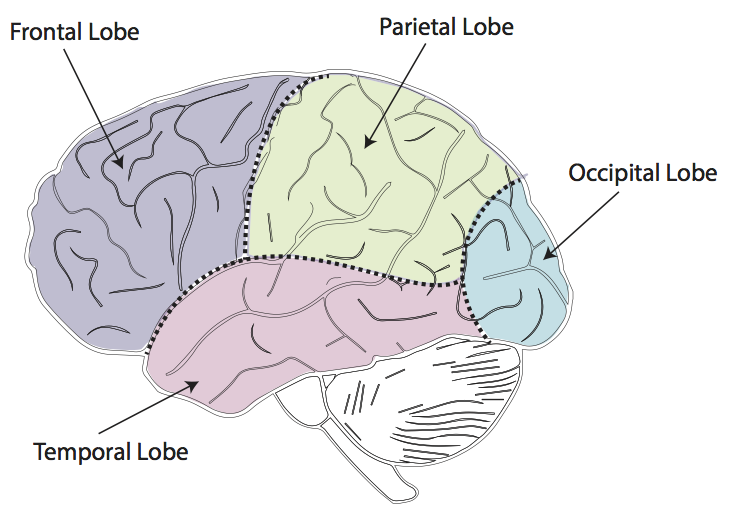
\includegraphics[width=.43\textwidth]{./images/brain_lobes.png}}
\hspace*{.2in}
\raisebox{-0.5\height}{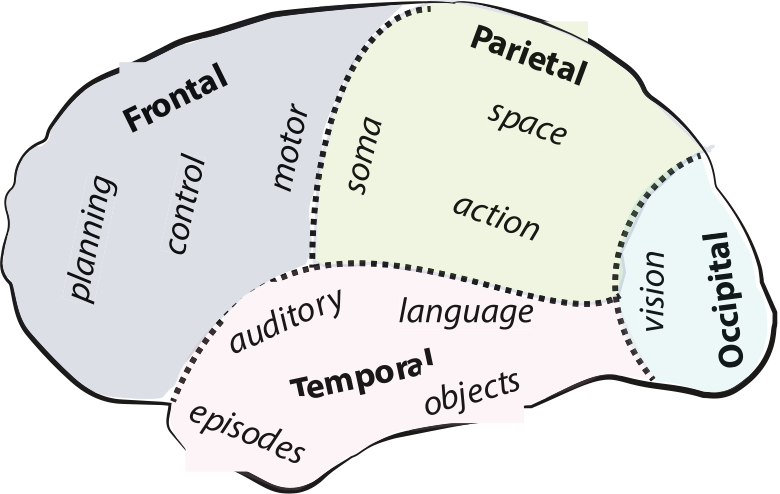
\includegraphics[width=.35\textwidth]{./images/brain_functions.png}}
\caption[Left: Pamela Payne; Right: Pamela Payne, using text taken from the Emergent Wiki.]{(Left) The lobes of the brain. (Right) Rough map of functions, abilities, and conceptual domains associated with major brain areas.}
\label{brain_lobes}
\end{figure}
% Right panel has a slight graphical error on top "dorsal" to the pic
% Add concrete/abstract, how -what, and an inset showing hot / cool, OFC, and ACC. Also redo 3.9 in a similar way

\subsection{Cortex}

Fig. \ref{brain_lobes} (Left) shows the major regions of the brain. Fig. \ref{brain_lobes} (Right) summarizes the functions associated with these areas. These are regions of the \glossary{cerebral cortex}, which is the wrinkled outer surface of the brain (cortex literally means ``rind'', like the outer skin of an orange or lemon). The wrinkling is caused by the cortex folding, like a crumpled piece of paper, in the limited volume of the skull. This folding results in bulges (called ``gyri'') and valleys (called  ``sulcuses'' or ``sulci'') on the surface of cortex. The cortex is thought to be involved in the higher processing functions distinctive of complex behavior and intelligent animals. The size of an animal's cortex roughly correlates with the complexity of its behavior and overall intelligence: humans and dolphins have a relatively large cortex, chimps a smaller cortex, rats even smaller, and non-mammals like birds and insects have no cortex at all. The cortex is composed of two hemispheres, the right and the left hemispheres, connected by a structure made up of nerve fibers called the ``corpus collosum''. Between-hemisphere communication occurs through the corpus collosum. In patients with a neurological disorder called ``epilepsy'', where too much neuronal firing in the brain leads to seizures, the corpus collosum is often severed (this is called a ``collosotomy'') to reduce between-hemispheric communication and prevent future seizures. Both the right and left hemispheres are made up of the same lobes (occipital, temporal, parietal, and frontal).	

From a computational standpoint, the cortex is the brain's primary long-term memory system, which stores all the many things we know about the world: how we classify objects, our concepts, our beliefs, our memories, our knowledge about our friends and family, our life goals and fundamental cares, almost everything is coded into this massive memory system. Many neural network models are directly or indirectly simulations of our long-term cortical memory system. They model pattern recognition via learning, memory storage and recall, pattern completion, spreading activation, and many other phenomena. In fact, unless otherwise noted, most neural networks are probably ultimately models of how cortex works.
% Mention cortex model in Simbrain
%It is like your persistent storage system, but it is quite different from a computer's solid-state memory at all. In a computer, memory is distinct from processing, but in the brain, the same circuits that support memory also support processing.  There are many disanalogies. In general, it is a living, pulsing, plastic tissue, a network of millions of cells and billions of synapses that are constantly being incrementally updated.  

The cortex has dense bi-directional recurrent connections that allow it to reverberate in sustained patterns. It  also has long range connections between areas that allow it to produce complex brain-wide patterns or oscillations (though some circuits are also similar to feed-forward networks). In concert with the central thalamic relay station (more on this below), the posterior and parietal parts of cortex reverberate and coordinate sensory input and motor outputs when you engage in most behaviors. The frontal regions manage our plans and actions. Other circuits refine these signals, producing smoother movements (cerebellum), coordinating sequences of activations to produce reward (basal ganglia), and managing recent memories (hippocampus). Thalamo-cortical oscillations are correlated with consciousness. When you see something and are aware of it,  sustained processing in multiple cortical areas is  associated with your experience: visual activations are associated with visual awareness, activation in somatic areas is associated with awareness of your body, more distributed activations are associated with inner thoughts, etc. These are sometimes referred to as the neural correlates of consciousness or NCCs.
% Add NCC citation
% Summarize GNW vs. RPT and expand on consciousness discussion, with citations.
% Even those who deny this, like Solms, allow that they are correalted

Learning in this long-term memory store occurs via a mixture of unsupervised and supervised learning. Synapses are updated by LTP and other means,  which can be modeled using unsupervised learning algorithms like Hebbian learning and unsupervised architectures such as self organizing maps (see chapter \extref{ch_unsupervised}). One theory of cortex is that it is a giant collection of internal models in long-term memory: models of physical objects, the people you know, language, etc. These models learn from unsupervised methods, but they also come to have expectations about external inputs and inputs from other models. On this view, most processing in the cortex, and thus most of what we see and hear and understand, is based on what we \emph{expect}, based on our internal models of situations. The signals that flow through cortex are actually error signals--a kind of training signal--which  indicate how what we see differs from what we expect. Thus cortical networks incorporate elements of supervised learning (chapter \extref{ch_supervised}). This view, known as the ``predictive coding'' or ``predictive processing'' view, originates in part in computational models of visual cortex \cite{rao1999predictive}, but it has since developed into a more general view about the structure of perception and cognition and their realization in the brain \cite{clark2013whatever}.
% More citations. Free energy etc. Also clarify that this is controversial.
% Top down vs. bottom up effects in perceptions
% Link to IAC HW. Think of all the things you can encode in an IAC network. But problem is that's not unsupervised.

In many cortical areas there is a progression from areas that handle low-level sensory processing (e.g. edge detection in primary visual cortex, or tones in primary auditory cortex) to regions that handle more complex pattern recognition, like face recognition. The reverse direction is similar: high level plans are handled by more ``interior'' networks, while detailed motor movements are handled closer to the output layers of the cortex, that feed to thalamus and then to muscle systems. Thus, many cortical areas have a hierarchical structure, which is precisely what is modeled by deep networks. 
% Check and improve esp this paragraph

\subsection{The Occipital Lobe}

The \glossary{occipital lobe} and some of its features are shown in Fig. \ref{brain_vision}. Its most dominant feature is the \glossary{visual cortex}, which supports visual processing, including edge detection, color detection, and simple motion detection. Damage to the visual cortex can produce blindness (\glossary{cortical blindness}), even if the eyes are intact. Processing begins in the eye (in the retina, which is itself a complex neural network), and is then passed along to several structures, most prominently the visual cortex. Processing within the visual cortex occurs in a series of stages, which are thought to correspond to the extraction of increasingly complex features of a visual scene. For example, V1 and  V2  process information about edges and form, V4 is involved in processing of color, and area MT plays a role in motion processing. 
% Mention Hubel / Wiesel?

\begin{figure}[h]
\centering
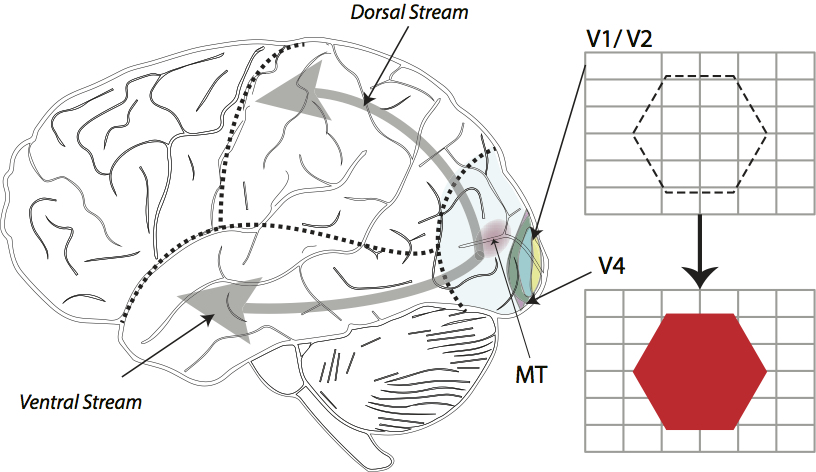
\includegraphics[scale=.6]{./images/brain_vision.png}
\caption[Pamela Payne.]{The visual cortex and associated structures.}
\label{brain_vision}
\end{figure}
% Add IT and FFA

% Clarify what a map is. Nearby firing neurons represent similar classes of inputs. Then use parallel constructions in discussion the other topographic maps.
Each of the regions of visual cortex contains something called a \glossary{retinotopic map}, which is a full neural map of locations in the retina, where groups of neurons nearest one another process information about nearby areas in visual space. More generally, a \emph{topographic map} is an area of the cortex where sensory information is processed in a spatially organized manner. We will see that multiple sensory regions contain topographic maps of their respective sensory information. In chapter \extref{ch_unsupervised} we will see that some neural network algorithms, like self organizing maps, can automatically produce banks of detectors that are topographically organized.

Information passes out of the visual cortex in two streams: a \glossary{dorsal stream} to the parietal lobe, which is involved in coordinating visual and spatial information, and a \glossary{ventral stream} to the temporal lobe, which is involved in processing complex visual features of objects and semantic knowledge, i.e. information about what things are  (see Fig. \ref{brain_vision}). We will discuss these pathways in more detail below.
% Object recognition is something many FF neural networks  do

\begin{figure}[h]
\centering
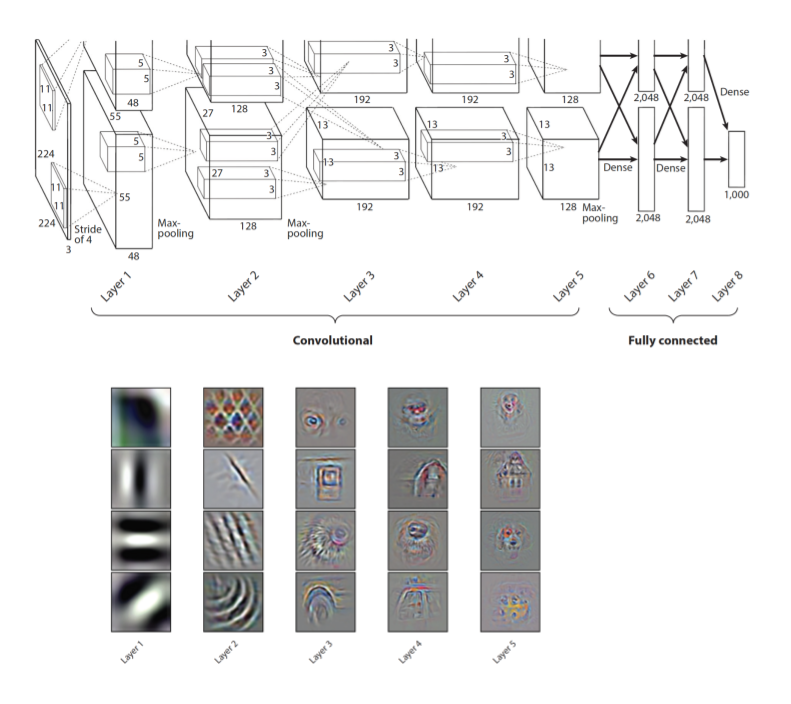
\includegraphics[scale=.4]{./images/deepLearningBrain.png}
\caption[From \cite{kriegeskorte2015deep}, which is in turn based on \cite{krizhevsky2012imagenet} and \cite{gucclu2015deep}.]{A well-known deep neural network architecture AlexNet (based on \cite{krizhevsky2012imagenet}) whose activations match those of actual brain areas. The top level shows the network architecture, and the bottom panel shows receptive fields (activations that maximally activate specific nodes) of a similar network \cite{gucclu2015deep}. Though these networks were developed as an engineering tool to classify images, they do a good job of describing neural activation in V1, V2, V4, and IT.}
\label{deepLearning_Vision}
\end{figure}
% This is misleading, because they are two networks. Also we need to get permissions.

It has emerged in recent years that deep learning networks are particularly well suited to describing what these areas of the brain do. These networks are trained to recognize images, which is a useful engineering application, but it turns out they do a good job of describing neural activity in the brain. For example, a well known deep network known as ``AlexNet'' \cite{krizhevsky2012imagenet} is shown in the top panel of figure \ref{deepLearning_Vision}. It develops topographic maps similar to those in the brain. The activations it produces at its various layers in response to images match the activations of the brain in response to the same images quite well. The earlier layers of the model mimic the response properties and receptive fields of lower levels of processing, like V1, and later layers mimic properties V4 and ventral stream neurons in IT. The exciting thing about these models is that we can produce pictures of their receptive fields, showing precisely what kind of input each neuron learned to respond to. As can be seen in the figure, lower level layers in this kind of network become edge detectors, further downstream layers respond to combinations of these features (compare Selfridge's demons from chapter \extref{ch_history}), while IT layers respond to dogs, cats, etc.\footnote{There has also been some skepticism about deep network approaches to human vision \cite{bowers2022deep}.}
% Principles apply in other brain areas

\subsection{The Parietal and Temporal Lobes}

% Clarify. Neurons are arranged spatially in a way that matches the arrangement of tones by frequency.
The \glossary{temporal lobe} is involved in auditory processing and semantic processing (see Fig. \ref{brain_audition}). The \glossary{auditory cortex} is in the temporal lobes. Much of the sensory information from the ears is sent to auditory cortex. Primary auditory cortex (A1) contains a \glossary{tonotopic map} of the acoustic properties of sounds. That is, neurons in this region respond to preferred frequencies of sound in a similar way to the preferred spatial regions in retinotopic maps. Auditory information is also processed in a somewhat hierarchical fashion, similar to vision. After A1, information passes to the secondary auditory cortex (A2), where sound localization and processing of more complex sound features occurs. When the auditory cortex is damaged, people can experience hearing deficits (they may suffer from ``central hearing loss'' or cortical deafness) even if the ears are intact. Other parts of the temporal lobe are involved in language processing. Wernicke's area, located in the temporal lobe\footnote{More specifically, the temporal lobe in the dominant hemisphere, which is usually the left hemisphere.}, plays an important role in speech understanding. This region is involved in assigning meaning to sounds. Damage to this area can produce \glossary{Wernicke's aphasia}, where patients are unable to understand either spoken or written language.
% Make cortical deafness a glossary item to match cortical blindness
% Some revision to bring out the sequence of processing centers

\begin{figure}[h]
\centering
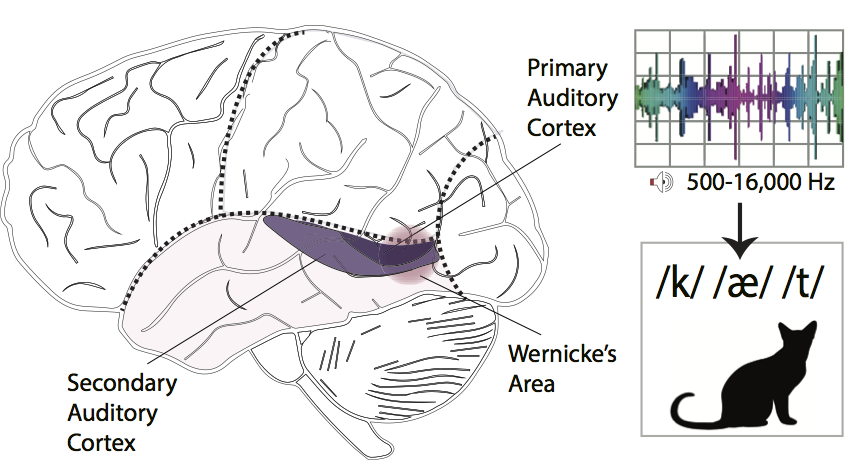
\includegraphics[scale=.7]{./images/brain_audition.png}
\caption[Pamela Payne.]{Auditory cortex and associated structures.}
\label{brain_audition}
\end{figure}
% Explain the phoneme symbols in the caption
% Add fusiform face area to image

The  temporal lobe also receives connections from the visual processing centers of the occipital lobe, via the ventral stream (Fig. \ref{brain_vision}). The ventral stream is involved in object recognition. For example, the fusiform face area (FFA) in the temporal lobes is connected with the recognition of faces. Damage to this region will cause \glossary{prosopagnosia}, an inability to recognize faces. It has since also been found that the FFA is active in bird experts while looking at birds and chess players while recognizing chess board configurations. This suggests that this region is involved in recognition of objects that one has expertise with \cite{boggan2011chess}. Another form of damage to the ventral stream can cause \emph{ideational apraxia}, where patients have difficulty interacting with objects because they can no longer understand what the object is used for. 
% Ref for FFA: Amy L. Boggan and Chih-Mao Huang, 2011
% Damage makes it hard to for example to identify an apple as an apple. This is a form of visual agnosia
% Ideational apraxia. .. sometimes called "semantic amnesia" of tool use
% This is the "bottom half" of temporal lobe. The top half has the more auditory stuff.

The \glossary{parietal lobe}, shown in Fig. \ref{brain_audition}, is involved in integrating information from multiple regions of the brain, as well as processing information about space. The dorsal stream carries spatial information from the occipital to the parietal lobe. It is involved in spatial attention, reaching, grasping, using tools, and other activities that coordinate visual information with motor behavior. Damage to regions of the parietal lobe can produce a number of problems. Patients with \glossary{hemineglect} tend to only pay attention to certain parts of the visual field. Such a person might only eat food one one side of their plate, or draw images on only one side of a page. It is said that a director who had hemineglect produced movies in which the action only happened on one side of the screen. Another form of damage to  the dorsal stream will cause \emph{ideomotor apraxia}, which results in difficulty using objects in space. Someone with ideomotor apraxia will have difficulty converting the idea of an action into the action itself. For example, they might have difficulty combing their hair when asked to do so, even if they can identify the hair brush and understand the function of the brush. The difficulty is in the execution of the action. This disorder highlights the role of the dorsal stream in coordinating action in space.
% This is illustrated abstractly by the braitenberg vehicles

The parietal lobe also receives tactile information from the body via the \glossary{somatosensory cortex} (Fig. \ref{brain_motor}), which in turn receives touch and temperature information processed by specialized mechano-receptors on the skin. When the somatosensory cortex is stimulated, people report feelings in specific parts of the body. The somatosensory cortex is a \glossary{somatotopic map}, in which nearby regions of neural tissues respond to pressure or temperature on nearby regions of the body. As shown in Fig. \ref{brain_motor}, more sensitive body parts are allocated more space in somatosensory cortex. For instance, the fingers and lips have greater cortical representation than other regions, while the shoulders and trunk have much less. In the somatosensory cortex of a mouse, almost all of the space is allocated to the whiskers, with each whisker receiving a relatively large amount of neuronal space. The primary somatosensory cortex is located right next to the primary motor cortex (discussed below), allowing for quick communication between these regions. 

\begin{figure}[h]
\centering
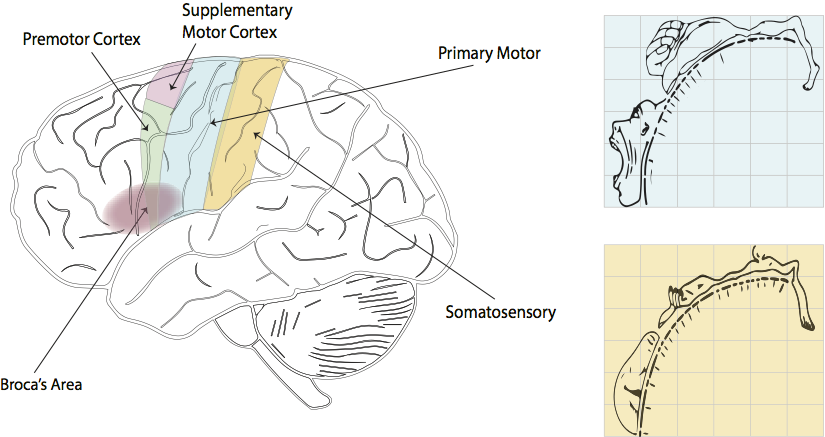
\includegraphics[scale=.8]{./images/brain_motor.png}
\caption[Pamela Payne.]{Somato-sensory and motor processing.}
\label{brain_motor}
\end{figure}
% Add "cortex" to somatosensory label and rearrange labels a bit

\subsection{The Frontal Lobe}
 
 % Cohere with what Chelsea says: ventro-medial planning, orbito frontal decision making
The \glossary{frontal lobe} is involved in higher-level cognitive functions, or \emph{executive functions}, like the ability to pay attention, select strategies, solve problems, plan actions, make decisions, inhibit or suppress behaviors, and in general control one's behavior. These functional associations rely upon a distributed network of regions including the orbito-frontal, dorso-lateral prefrontal, and ventro-medial areas.\footnote{The \emph{Ventro-medial prefrontal cortex} has been shown to be involved in the representation of the internal state of the body and the relative value of decisions. \emph{Orbito-frontal cortex} is also involved in decision-making and is thought to play a particular role in assessing reward.} The rear-most parts of the frontal lobe, like the \glossary{primary motor cortex}, are directly involved in action. In fact, the frontal lobes can be thought of as controlling action on a spectrum from specific movement in the primary motor cortex to  increasingly abstract planning and decision making in the front-most parts of the cortex, like the orbito-frontal cortex. Some language processing also takes place in the frontal lobe. \glossary{Broca's area} (Fig. \ref{brain_motor}) is responsible for many language functions, including gesture, understanding of action and action-language, and language production. 

\begin{figure}[h]
\centering
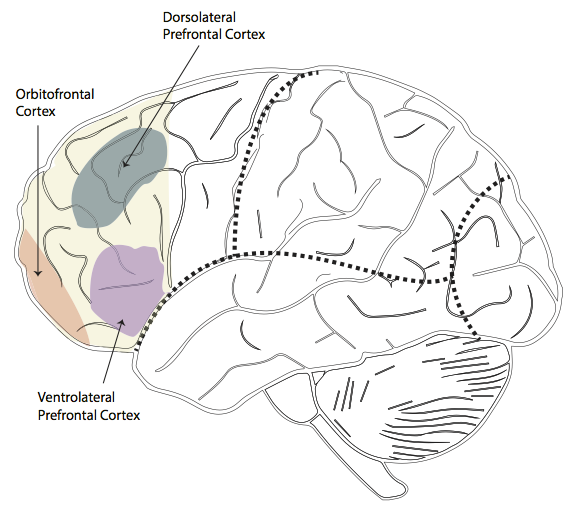
\includegraphics[scale=.75]{./images/brain_frontal.png}
\caption[Pamela Payne.]{The prefrontal cortex.}
\label{brain_frontal}
\end{figure}
% Change the VLPFC to VMPFC in picture and in label.

The parts of the frontal lobe closer to the center of the brain are directly involved in controlling the body. Neural outputs to the body originate in the \glossary{primary motor cortex} (see Fig. \ref{brain_motor}). When parts of the primary motor cortex are stimulated people contract the relevant muscles of their body. When \emph{premotor cortex} is stimulated, people will actually start to make complex movements, such as grasping. \emph{Supplementary motor cortex} is less well understood and does not include a map of the body in humans, but this region is thought to play an important role in coordinating movement plans, in particular sequences of movements.

The dorso-lateral \glossary{prefrontal cortex} or PFC is associated with working or short-term memory. It is part of the cortex but has evolved a distinctive structure that supports the unique demands of working memory. Its cells are relatively isolated from other areas, but with dense recurrent connections that facilitate a particular type of neural dynamics, an ``attractor structure'' (see chapter \extref{ch_dst}), whereby activations tends to settle into stable patterns for a time, which are maintained in cortical ``stripes'' \cite{kriete2013indirection}. These stripes are thought to encode task information in working memory. Your current plans and goals are maintained by active stripes in your PFC. As you go through your day doing one thing after another--making breakfast, driving to school, reading a book, etc.--different stripes corresponding to current goals are sequentially activated in PFC. Support for this idea is provided by experiments that show that while humans and monkeys maintain goals to look or reach in different directions, specific populations of neurons are active in the PFC. In some neural network models, actively maintained tasks are simulated simply by clamping certain nodes in the on or off position. For example, one node might correspond to reading letters, while another might correspond to saying what color the letters are written in, in a model of a task where you can either read letters or say their color.\footnote{These are models of the Stroop effect; see \url{https://en.wikipedia.org/wiki/Stroop_effect}}
% Add Simbrain Stroop network reference
% Add the reference to the empirical literature

% Citations needed
% Primary motor regions process simple movement, while premotor regions are involved in complex goal-based movement, while further forward information about higher goals is integrated. 
% Broca's aphasia isn't  mentioned...
% Give examples of broca's and wernickes aphasia?  E.g. from wiki example of broca's or expressive aphasia speech:  "Yes... ah... Monday... er... Dad and Peter H... (his own name), and Dad.... er... hospital... and ah... Wednesday... Wednesday, nine o'clock... and oh... Thursday... ten o'clock, ah doctors... two... an' doctors... and er... teeth... yah.[10]"

 Damage to the frontal lobe results in a variety of deficits, including difficulties with impulse control, impaired judgment, personality abnormalities, and an inability to make any decisions at all. A famous case of damage to the frontal lobe is provided by Phineas Gage, a 19th century railroad worker whose skull was pierced by a large iron rod in an explosion. Once the iron rod was removed, Gage retained full cognitive function, and the only prominent change was in his behavior. After the surgery, he had a more difficult time inhibiting certain behaviors, became more hostile, drank excessively, and eventually became homeless.

\subsection{Other Neural Networks in the Brain }

We have been focusing on the cortex, which is by far the most dominant structure in the brain. Many neural network models are basically modeling cortex and how it extracts features from sensory inputs layer by layer, maintains task information in the frontal areas, etc. These are models of different aspects of long-term memory. However, there are also many other specialized circuits that have been modeled by distinctive forms of neural network model. See figure \ref{brain_internal} for an overview of the structures we discuss here.

\begin{figure}[h]
\centering
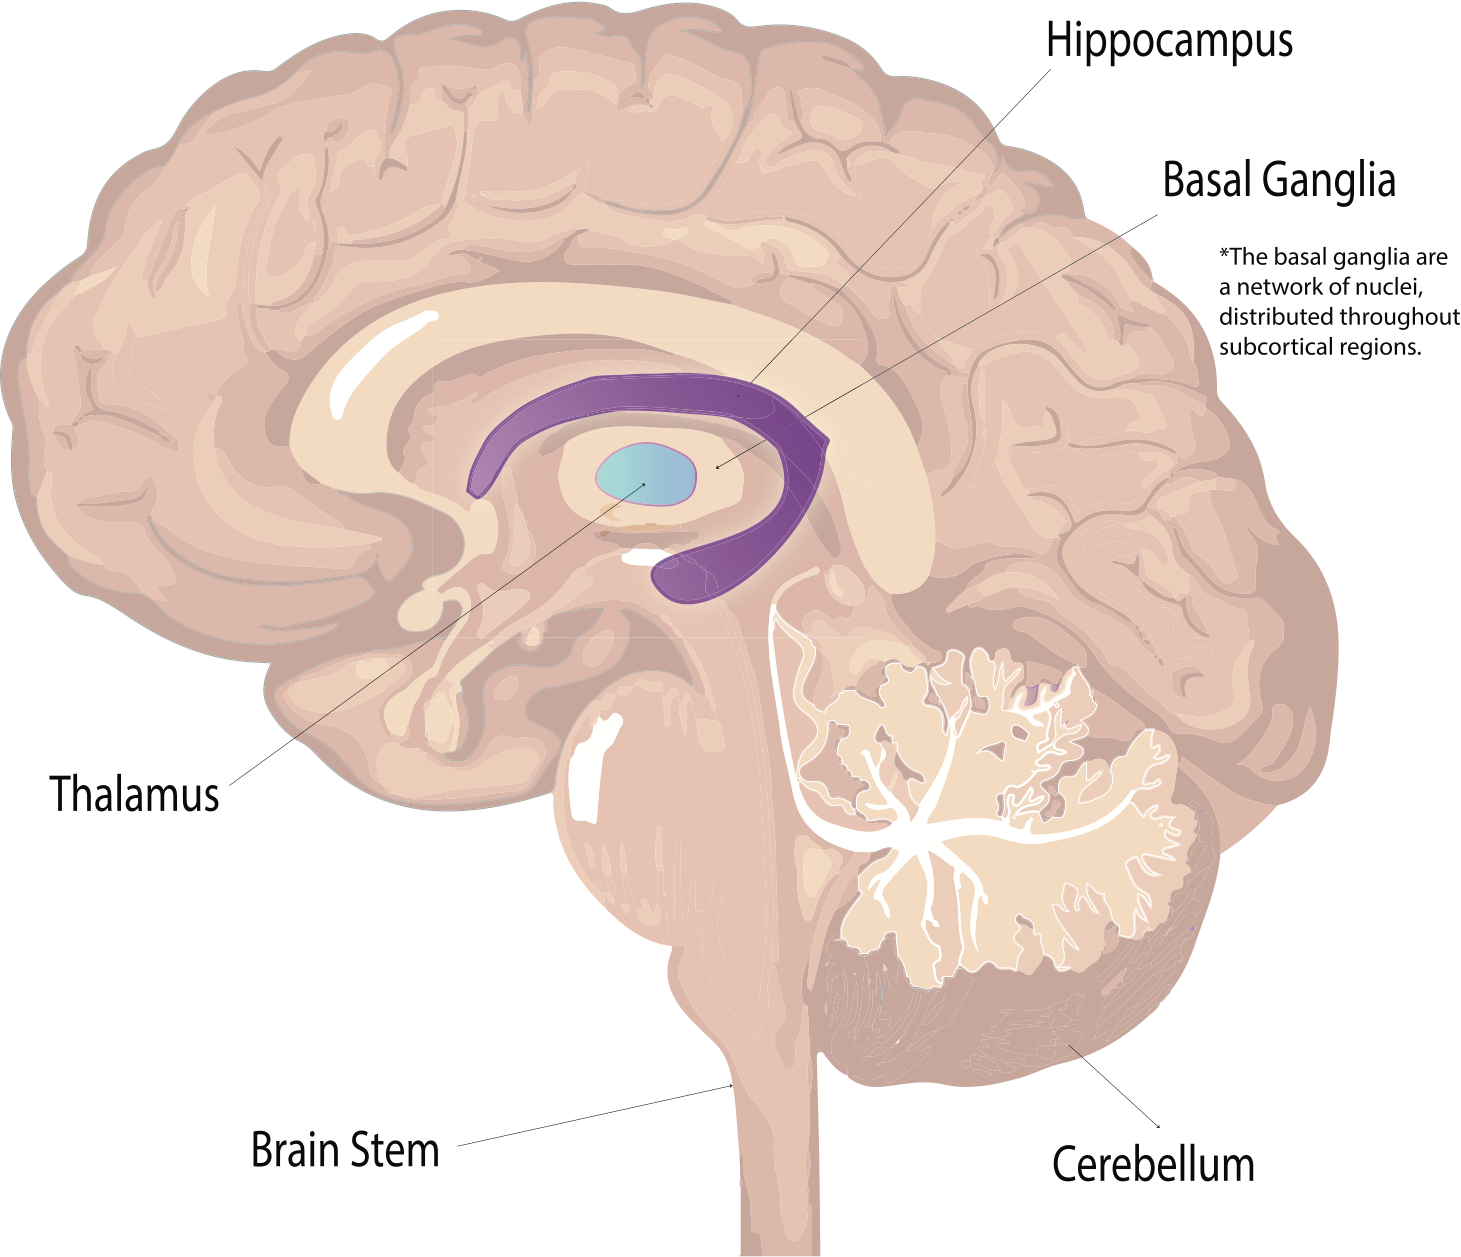
\includegraphics[width=.5\textwidth]{./images/brain_internal.png}
\caption[Pamela Payne.]{Some specific structures in the brain with specific neural network structures.}
\label{brain_internal}
\end{figure}

% Below should add retrograde amnesia and explain the difference
% Episodic memories more in hippocampus
The \glossary{hippocampus} is a kind of short-to-medium-term memory system attached to the bottom of the cortex.\footnote{In fact it is directly attached to the temporal lobes, and is hard to see as being separate on visual inspection, but its neurons are arranged differently than the neurons in the cortex.} It is associated with memory consolidation, spatial memory, and episodic memory. It has a special neural network structure that allows it to watch what is happening in the cortex, and then build up special ``sparse coded'' representations.\footnote{For simulation-based tutorials on computational models of hippocampus see \url{https://compcogneuro.org/}.}  While learning in the cortex is slow, learning in the hippocampus is fast. It can pick up all the things that happen in your day and remember them for a few weeks or even longer. These memories don't always last, and in fact new neurons are constantly being created in hippocampus (it's one of the few parts of the brain where neurogenesis continues into adulthood). Dreams are thought to be mediated by hippocampus, which is why dreaming often involves recent events. When things get repeated enough in hippocampus, they are consolidated into the cortex. It's like it learns a fast representation, and then that either evaporates or if repeated enough, gets transferred to cortex. Damage to the hippocampus can produce various forms of amnesia, e.g. \glossary{anterograde amnesia}, now familiar via movies like \emph{Memento}, where characters live entirely in the present and cannot remember things that they learn after the date of their injury. Interestingly, patients with this form of amnesia are often able to create new \emph{procedural memories}, such as a ``memory'' of how to ride a bike, but are unable to create any new episodic, semantic, or fact-based memories, such as memories of events in the news. Neural network models of hippocampus have been used to study how memories can be consolidated into long term memory. The models can, for example, be used to simulate amnesia.
% Also spatial maps of the environment
% Citations

 The \glossary{basal ganglia} is an important collection of nuclei beneath the cortex which have a variety of functions, including (in concert with pre-frontal cortex) control of voluntary action, and learning how to take actions that are likely to lead an agent to rewarding stimuli. It is thought to implement a form of \glossary{reinforcement learning}, whereby actions that produce reward tend to be reinforced over time, and actions that produce costly outcomes are inhibited (this formalizes older ideas in psychology about operant conditioning). It's a bit like a task scheduler or sequencer, orchestrating extended sequences of activations in the cortex. It is also thought to be involved in deciding what tasks and goals should be loaded into the frontal areas of the brain, determining what tasks are maintained in PFC's stripes, and in what sequence. It implements reinforcement learning in part using the neuromodulator dopamine, discussed above. These same reinforcement learning techniques have also been shown to work well in machine learning.\footnote{Reinforcement learning was, for example, used in Alpha Go (mentioned in chapter \extref{ch_intro}), the first neural network to beat a professional human Go player \url{https://deepmind.com/research/alphago/}} In fact, there was a great deal of excitement in the 1990s when it was first discovered that dopamine neurons in the basal ganglia responded to rewards in the same way as certain variables in reinforcement learning models: more activity when reward is higher than expected; less activity when reward is less than expected  \cite{schultz1997neural, niv2009reinforcement}.  When things go better than we expect, dopamine is released, and synapses are strengthened, reinforcing whatever we have done recently, making us more likely to do the same thing in the same situation in the future. Thus the dopamine system and the basal ganglia ``sequencer'' learns to execute sequences of goals and actions that tend to produce reward in the long run and avoid punishment.\footnote{Some of these ideas can be studied using the actor-critic model in Simbrain (available from the simulation menu). Links to operant conditioning can be studied using the Rescorla-Wagner and operant conditioning simulations).  The relation to frontal lobes and task maintenance is explored in CECN models at \url{https://compcogneuro.org/}.}
% Glossary for  dopamine, mid-brain?
% More citations
 
\begin{figure}[h]
\centering
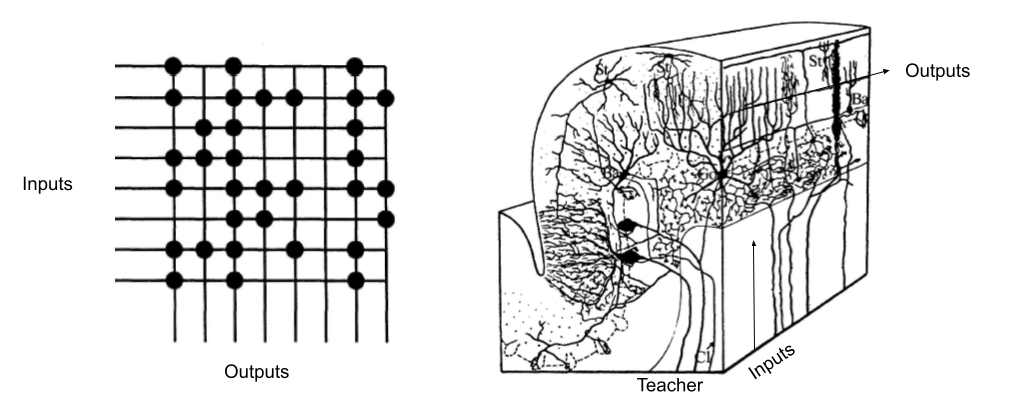
\includegraphics[scale=.3]{./images/cerebellum_Associator.png}
\caption[From lecture slides by David Touretsky.]{The cerebellum as a pattern associator, mapping sensory states to motor actions. (Left) An input-output architecture: synapses where input lines and output lines overlap can be turned on when a teacher signal turns on. (Right) Associated areas of the cerebellum thought to correspond to these functions.}
\label{cerebellum_associator}
\end{figure}
% Get original figure attributions and add citation.
% Add arrows to the figure!

The \glossary{cerebellum} is involved in fine motor control (it also has cognitive functions but these are less well understood). When it is damaged, movement becomes jerky and ballistic (\glossary{ataxia}). Neural network models treat the cerebellum as a massive pattern associator, or even as a neural ``lookup table''. It has a structure that made it an attractive target for computational neuroscientists in the late 1960s and early 1970s \cite{marr1991theory}. As can be seen in figure \ref{cerebellum_associator}, it receives many inputs and produces many outputs, and there are also neurons that seem to climb up and surround certain neurons, suggesting that they carry an error signal used to update certain synapses. This led to the idea that it was a pattern associator trained by supervised learning, a theory which remains popular, though the issue is not settled. One thing it certainly does is learn to associate bodily and sensory inputs with motor outputs, which helps produce rapid and smooth action sequences. It's as if the coarse-grained motor plans produced by the cortex and basal ganglia are ``smoothed'' by this cerebellar associative map.

The \glossary{thalamus} is a subcortical region responsible for  processing and relaying information between the cortex and  sensory and motor structures on the body. Information from most  sensory modalities passes through the thalamus on the way to the cortex. It is sometimes called the ``gateway to the cerebral cortex.''  Recurrent loops between the thalamus and cortex (\emph{thalamo-cortical loops}) produce wide-spread synchronized patterns of activity in the cerebral cortex which are, as noted above, associated with conscious experience.

Finally, more fundamental functions of the brain, like the control of the lungs, heart, and sleep, take place in the \glossary{brain stem}. Damage to the brain-stem often results in death.
% Draw on Solms and Damasio. Homeostasis. Also how we can be cs without cortex but still be situationally and affectively responsive.

